\documentclass[a4paper]{article}
\usepackage[ngerman]{babel}
\usepackage[T1]{fontenc}
\usepackage[utf8]{inputenc}
\usepackage{pdfpages}
\usepackage{a4wide}
\usepackage{amsmath}
\usepackage{amssymb}
\usepackage{graphics}
\usepackage{mathrsfs}
\usepackage{xspace}
\usepackage{verbatim}
\usepackage{float}
\usepackage{csvsimple}
\usepackage{pgfplotstable} % Generates table from .csv
\usepackage{setspace}
\usepackage{currfile}
\usepackage{subcaption}
\usepackage{gensymb}
\usepackage{amsmath}
\usepackage{tabularx}
\restylefloat{table}
\providecommand{\zB}{z.\,B.\@\xspace}
\providecommand{\Matlab}{\textsc{Matlab}\xspace}
\usepackage[binary-units]{siunitx}
\sisetup{locale = DE}
\sisetup{per-mode = symbol-or-fraction}
\DeclareSIUnit\rounds{U}
\DeclareSIUnit\nmeter{Nm}
\usepackage[breaklinks=true]{hyperref}
\def \Stator {S}
\def \Rotor {R}
\renewcommand{\j}{\jmath}
% Ableitungen
\newcommand{\dd}{\mathop{}\!\mathrm{d}}
\newcommand{\Diff}[2]{\frac{\dd#1}{\dd#2}}
\newcommand{\DiffT}[1]{\Diff{#1}{t}}
\newcommand{\DDiff}[2]{\frac{\dd^2#1}{\dd#2^2}}
\newcommand{\DDiffT}[1]{\DDiff{#1}{t}}
\newcommand{\PartDiff}[2]{\frac{\partial #1}{\partial #2}}
\newcommand{\PartDiffT}[1]{\Diff{#1}{t}}
\newcommand{\PartDDiff}[2]{\frac{\partial^2 #1}{\partial #2^2}}
\newcommand{\PartDDiffT}[1]{\DDiff{#1}{t}}

% Makro für Gleichungen, Abbildungen, Tabellen
\newcommand{\abb}[1]{Abb. \ref{#1}}
\newcommand{\tab}[1]{Tab. \ref{#1}}
\newcommand{\glg}[1]{Glg. \ref{#1}}
\newcommand{\chp}[1]{Kap. \ref{#1}}
\usepackage[european]{circuitikz}
\usepackage{tikz}
\usetikzlibrary{arrows,decorations,intersections, decorations.text,calc}
\usepackage{pgfplots}
\pgfplotsset{compat=1.15}
\usepgfplotslibrary{units}
\pgfplotsset{ticklabel style={/pgf/number format/use comma,/pgf/number format/1000 sep={ }}}
\usetikzlibrary{external,arrows}
\tikzexternalize[prefix=tikz/,optimize command away=\includepdf]
\tikzset{external/up to date check=simple}
\tikzset{external/force remake}
\begin{document}
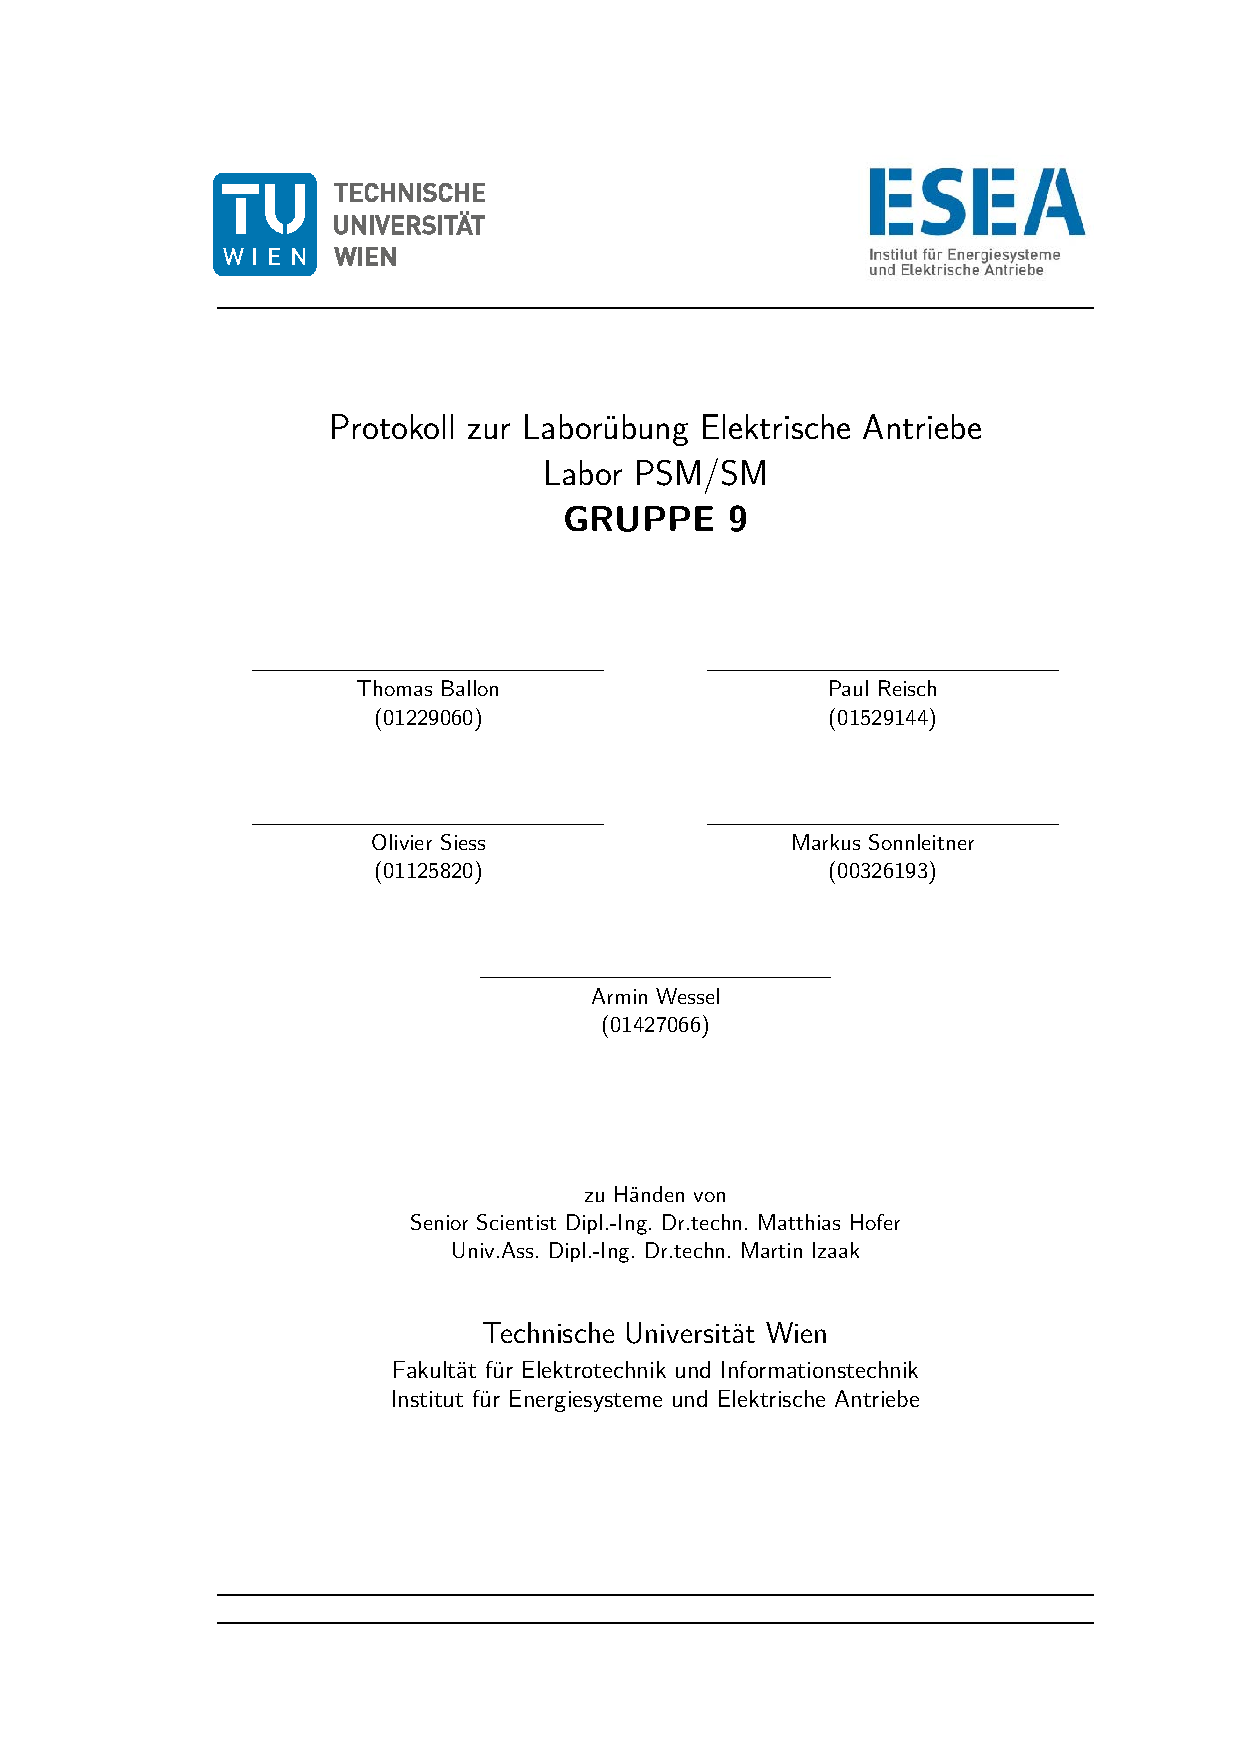
\includepdf{Deckblatt_PSM}
\tableofcontents\newpage
\include{Einleitung}

%SM
\section{Elektrisch erregte Synchronmaschine}
Die in der Laborübung verwendete Maschine besitzt jeweils 3 Wicklungen pro Strang. Die Wicklungen können wahlweise am Klemmkasten seriell oder parallel und in Stern oder Dreieck verschaltet werden. Für die Übungsdurchführung wurden die Wicklungen seriell in Stern geschaltet, wodurch sich folgende Nenndaten ergeben:
\begin{equation*}
    U_N=\SI{400}{\volt}, \quad I_N = \SI{57.7}{\ampere}, \quad n_N = 1000\,\frac{\textrm{U}}{\textrm{min}}
\end{equation*}
Eigentlich handelt es sich dabei um eine Schenkelpolmaschine (Achsigkeit), allerdings wird diese für unsere Zwecke als Vollpolmaschine behandelt. Außerdem besitzt die Synchronmaschine eine gekoppelte Nebenschlussmaschine, welche den Erregerstrom für die Synchronmaschine liefern kann. Somit kann das System im Fall eines Blackouts ohne externe Versorgung (Erregung) hochgefahren werden. Für unsere Anwendung wurde jedoch ein Spartransformator mit einem Gleichrichter für die Erregung verwendet.\\
Die elektrisch erregte Synchronmaschine (SM) ist mechanisch an eine Gleichstrommaschine (GSM) gekoppelt. Dabei handelt es sich um eine Nebenschluss-Gleichstrommaschine, die über ein starres Gleichspannungsnetz (Batterie) versorgt wird (siehe Abbildung\;\ref{fig:SM_Ueberblicksschaltung}). Beim Einschalten ist darauf zu achten, dass der Einschaltstrom durch einen Anlaufwiderstand $R_V$ begrenzt wird, um eine Beschädigung der Laboreinrichtung (Maschine, Zuleitungen, etc.) zu vermeiden. Nachdem die Maschine hoch gefahren ist, wird der Anlaufwiderstand kurzgeschlossen und die Erregung über den Erregerwiderstand $R_E$ eingestellt (für den Anlaufvorgang wird $R_E$ auf ein Minimum eingestellt, um bei gegebenem Ankerstrom $I_A$ maximales Anzugsmoment zu erhalten).
\begin{figure}[htb]
    \centering
    \includegraphics[width = 0.85\textwidth, angle=0]{\currfiledir SM_Ueberblicksschaltung}
    \caption{Schaltungsaufbau der Synchronmaschine (SM) mit Antriebsmaschine (Nebenschluss-Gleichstrommaschine, GSM).}
    \label{fig:SM_Ueberblicksschaltung}
\end{figure}
\subsection{Leerlaufversuch}
\label{subsec:leerlauf}
\begin{figure}
    \centering
    \includegraphics[width=0.85\textwidth, angle=0]{\currfiledir SM_Leerlauf}
    \caption{Schaltungsaufbau zur Ermittlung der Leerlaufkennlinie der Synchronmaschine (SM).}
    \label{fig:SM_Leerlauf}
\end{figure}
Beim Leerlaufversuch der SM wird ein stromloser Stator und eine konstante Drehzahl $n=n_N$ vorausgesetzt. Gemessen wird die in den Statorwicklungen induzierte Spannung (=Klemmenspannung $U_{sL}$) in Abhängigkeit des Felderregerstroms $I_f$ dar. Letzterer wird ausgehend von $I_f=0$ erhöht, bis sich eine Klemmenspannung von $U_{sL}\approx\SI{500}{\volt}$ einstellt (1. Leerlaufmessreihe) und anschließend wieder bis $I_f=0$ reduziert (2. Leerlaufmessreihe).\\
Die Drehzahl wird über die (mechanisch) gekoppelte GSM auf eine Drehzahl von $n=n_N$ geregelt. Dazu wird die Erregung der Nebenschluss-GSM über den Vorwiderstand $R_E$ im Erregerkreis varriert bis sich die gewünschte Drehzahl einstellt und dort während der gesamten Messung gehalten. Die resultierende Leerlaufkennlinie ist in Abbildung \ref{abb:SM_Leerlaufkennlinie} zu sehen. Der charakteristische Felderregerstrom $I_{fL}$, für den
\begin{equation*}
    \frac{U_{sL}(I_{fL})}{U_{sN}} = 1 
\end{equation*}
gilt, entspricht $\approx\SI{4.5}{\ampere}$. Die aufgenommenen Messwerte sind im Anhang in Tabelle \ref{tab:SM_leerlauf} dargestellt.
\input{\currfiledir leerlauf.tex}

% \subsection{Kurzschlussversuch} 
Der Kurzschlussversuch der Synchronmaschine erfolgt mit kurzgeschlossenen Statorklemmen und (wie beim Leerlaufversuch) mit konstanter Nenndrehzahl $n=n_N$. Der Kurzschlussstrom wird mit einer Stromzange gemessen, während der Erregerstrom $I_f$ gesteigert wird. \\
Die Nenndrehzahl wurde wieder über die gekoppelte fremderregte GSM eingestellt und bei Bedarf nachgeregelt, sodass die Drehzahl über die gesamte Messung konstant bleibt. Die gemessene Kurzschlusskennlinie ist in Abbildung \ref{abb:SM_Kurzschluss} dargestellt. Der Zusammenhang ist linear, da die innere Spannung der Synchronmaschine aufgrund der Ankerrückwirkung wesentlich kleiner als die Nennspannung der Maschine ist. Die mittlere Steigung der Geraden lässt sich einfach über die gemeseenen Werte berechnen:
\begin{equation*}
    k_K = \frac{dI_{sK}}{dI_f} = \frac{60.5 - 0.7}{4.6 - 0} = 13
\end{equation*}
Dies entspricht bezogen auf den Nennstrom ca. $0.2253$. Der chrakteristische Felderregerstrom $I_{fK}$ entspricht der Gleichung 
\begin{equation*}
    \frac{I_{sK}(I_{fK})}{I_{sN}} = 1
\end{equation*}
und ergibt ca. $I_{fK} = \SI{4.44}{\ampere}$ und ist in der Abbildung ebenfalls eingezeichnet. Die aufgenommenen Messwerte sind im Anhang in Tabelle \ref{tab:SM_kurzschluss} dargestellt.
% TODO es ist nicht eingezeichnet
\input{\currfiledir kurzschluss.tex}

% \subsection{Synchronisation an das Spannungsnetz}
Im nächsten Schritt muss die Synchronmaschine mit dem Netz synchronisiert werden. Dabei müssen folgende Bedingungen für ein stoßfreies Zuschalten erfüllt werden:
\begin{itemize}
    \item gleiche Spannungsamplituden
    \item gleiche Frequenz
    \item gleiche Phasenlage
    \item gleiche Phasenfolge
\end{itemize}
Für die Bestimmung bzw. das Einstellen der richtigen Phasenlage bzw. Phasenfolge wird eine Hell-Dunkel-Schaltung verwendet (siehe Laborskript). Der Aufbau im Labor hat jeweils 3 redundante Lampen, um ein falsches Zuschalten aufgrund fehlerhafter Glühbirnen zu verhindern.\\
Die Spannungsamplitude wird über ein Voltmeter überprüft und gegebenenfalls mit dem Erregerstrom der Synchronmaschine entsprechend angeglichen.\\
Der Frequenzabgleich ist dann gegeben, wenn die Helligkeit der Lampen sich nicht ändert. Bei einer Frequenzdifferenz  stellt sich eine fortlaufende Spannungsänderung ein, die über die Lampen visualisiert wird (umlaufende "Dunkellampe"). Da bei der Synchronmaschine die Frequenz der Klemmenspannung in direktem Zusammenhang mit der Drehzahl der Maschine steht, kann die Frequenz über die gekoppelte GSM angepasst werden (durch Änderung der Erregung).\\
Die Phasenfolge ist dann gleich, wenn die ''richtigen'' Lampen hell bzw. dunkel sind. Bei Vertauschen der Phasenlage würden die falschen Lampen hell/dunkel sein. Dann kann zwar die Phasenlage übereinstimmen, die Phasenfolge allerdings z.B. $120^{\circ}$ verschoben sein, was einer umgekehrten Drehrichtung entsprechen würde. Ist die Phasenfolge nicht gleich, muss die Drehzahl kurzzeitig geändert werden, damit sich die beiden Drehspannungssysteme (starres Netz bzw. Synchronmaschine) zueinandereinander verschieben können.\\
Erst wenn alle Bedingungen erfüllt sind, kann die Maschine über einen Schalter mit dem Netz verbunden werden.

 \subsection{Bestimmung der Potierreaktanz}
\label{subsec:potierreaktanz}
\begin{figure}
    \centering
    \includegraphics[width=0.85\textwidth, angle =0]{\currfiledir SM_Leistungsmessung}
    \caption{Schaltungsaufbau (Ausschnitt) zur Leistungsmessung - Ermittlung des induktiven Volllastpunktes.}
    \label{fig:SM_Leistungsmessung}
\end{figure}
Nachdem die Maschine erfolgreich ans Netz gekoppelt wurde, wird die Potierreaktanz mit der graphischen Methode nach Fischer-Hinnen bestimmt.\\
Zusätzlich zur Leerlauf- und Kurzschlusskennlinie wird noch der induktive Volllastpunkt $IV$ benötigt, damit alle relevanten Maschinendaten bestimmt werden können. Der Induktive Volllastpunkt ist dadurch gekennzeichnet, dass die Maschine keine Wirkleistung sondern nur Blindleistung umsetzt. Die Maschine wirkt also kapazitiv aus Sicht des Netzes.\\
Um die Synchronmaschine in den induktiven Volllastpunkt zu bringen, wurde der Erregerstrom erhöht bis sich Nennstrom und Nennspannung einstellen. Die Verluste der Synchronmaschine werden von der GSM gedeckt, indem das Drehmoment (bzw. der Erregerstrom der GSM) so gewählt wird, dass keine Wirkleistung aufgenommen wird. Der induktive Volllastpunkt ist in Abbildung \ref{abb:Fischer_Hinnen} dargestellt und liegt bei ca. $I_{fIV} = \SI{10.4}{\ampere}$. Den Schaltungsaufbau bzw. dessen Aussschnitt für die Leistungsmessung (2-Wattmeter-Methode) stellt Abbildung\;\ref{fig:SM_Leistungsmessung} dar.\\
Für die Bestimmung der Potierreaktanz (nach der Methode von Fischer und Hinnen) muss nun der Strom $I_{fK}= \SI{4.4}{\ampere}$ vom Strom $I_{fIV}$ subtrahiert werden und ins Diagramm eingetragen werden. Durch Parallelverschiebung der Anfangssteigung der Leerlaufkennlinie durch eben erhaltenen Punkt, kann mit dem Schnittpunkt der Leerlaufkennlinie die innere Spannung im induktiven Volllastpunkt $u_{iIV} = 1.163$ abgelesen werden. Die Höhe des entstanden Dreiecks entspricht der Potierreaktanz $x_p = 0.163$. Die Teillänge $I''_{sN}= \SI{4}{\ampere}$ wird für die Berechnung des Umrechnungsfaktor $\gamma$ benötigt:
\begin{equation*}
    \gamma = \frac{I''_{sN}}{I_{sN}} = 0.069.
\end{equation*}
Dieser Faktor gestattet es, Statorströme auf äquivalente Felderregerströme - und umgekehrt - umzurechnen. Die Äquivalenz bezieht sich hier auf die dadurch entstehende Durchflutung bzw. der Amplituden der Grundwellen der magnetischen Flussdichte. D.h. es werden Felderregerströme (Gleichstrom) und Statorströme (Wechselstrom) in Beziehung zueinander gesetzt.\\
Darüber hinaus lassen sich das gesättigte ($k_ {c}$) und ungesättigte ($k_ {c0}$) Leerlauf-Kurzschluss-Verhältniss graphisch ablesen.
\begin{equation*}
    k_ {c0} = \frac{I_{f0}}{I_{fK}} = \frac{\SI{2.6}{\ampere}}{\SI{4.4}{\ampere}} = 0.59, \quad k_ {c} = \frac{I'_{f0}}{I_{fK}} = \frac{\SI{4.53}{\ampere}}{\SI{4.4}{\ampere}} = 1.03
\end{equation*}
Aus diesen können die gesättigte und die ungesättigte bezogene synchrone Längsreaktanz abgeleitet werden:
\begin{equation*}
    x_d = \frac{1}{k_c} = 1.69, \quad x_{d0} = \frac{1}{k_{c0}} = 0.97.
\end{equation*}
Die charakteristischen Ströme können durch die Beziehung
\begin{equation*}
    i_f = \frac{I'_f}{I_{sN}} = \frac{I_f}{\gamma I_{sN}}
\end{equation*}
auf die Statorseite umgerechnet werden. Die aus dem Diagramm entnommenen Werte sind in Tabelle \ref{tab:Fischer_Hinnen_abgelesene_Werte} zusammengefasst, die daraus berechneten Werte können der Tabelle \ref{tab:Fischer_Hinnen_berechnete_Werte} entnommen werden.

% Tabelle der abgelesenen Werte
\begin{table}[!ht]
\centering
\begin{tabular}{|c|c|}
\hline
            & abgelesene Werte      \\ \hline
$I_{fK}$    &  \SI{4.4}{\ampere}    \\ \hline
$I_{fL}$    & \SI{4.53}{\ampere}    \\ \hline
$I_{fIV}$   & \SI{10.4}{\ampere}    \\ \hline
$I''_{sN}$  & \SI{4}{\ampere}       \\ \hline
$x_p$       & $0.163$               \\ \hline
$u_{iIV}$   & $1.163$               \\ \hline
$u_{iK}$    & $0.163$               \\ \hline
$k_c$       & $0.59$                \\ \hline
$k_{c0}$    & $1.03$                \\ \hline
\end{tabular}
\caption{Grafisch ermittelte Werte aus LL- und KS-Versuch nach Fischer-Hinnen}
\label{tab:Fischer_Hinnen_abgelesene_Werte}
\end{table}

% Tabelle der berechneten Werte
\begin{table}[!ht]
\centering
\begin{tabular}{|c|c|}
\hline
            & berechnete Werte  \\ \hline
$i_{fK}$    &  $1.105$          \\ \hline
$i_{fL}$    & $1.137$           \\ \hline
$i_{fIV}$   & $2.612$           \\ \hline
$x_d$       & $1.69$            \\ \hline
$x_{d0}$   & $0.97$            \\ \hline
\end{tabular}
\caption{berechnete charakteristische Größen}
\label{tab:Fischer_Hinnen_berechnete_Werte}
\end{table}
\noindent Die synchrone Hauptfeldreaktanz $x_{dh}$ wurde abschließend als Funktion des bezogenen Magnetisierungsstroms $i_{md}$ bestimmt. Es gilt allgemein
\begin{equation*}
    \label{eq:Hauptfeldreaktanz}
    x_{dh} \big|_{i_{md}} = \frac{u_{iq} \big|_{i_{md}}}{i_{md}}
\end{equation*}
Der bezogene Magnetisierungsstrom ist durch 
\begin{equation*}
    i_{md} = i_f + i_{sd}
\end{equation*}
gegeben. Für den Leerlauffall gilt $i_s = 0 \rightarrow i_{sd} = 0$ und somit vereinfacht sich Gleichung \ref{eq:Hauptfeldreaktanz} zu:
\begin{equation*}
        x_{dh} \big|_{i_{f}} = \frac{u_{s} \big|_{i_{f}}}{i_{f}}
\end{equation*}
Der Verlauf der Hauptfeldreaktanz $x_{dh}$ ist im linearen Bereich der Leerlaufkennlinie konstant. Für steigende Felderregerströme $I_f$ kommt es durch die Sättigung des Eisens (Hauptfeldreaktanz sinkt) zu einer Abflachung der Leerlaufkennlinie. Im Bereich hoher Sättigung ist die Leerlaufkennlinie wieder annähernd linear, wodurch auch der Verlauf der Hauptfeldreaktanz wird wieder näherungsweise konstant verlaufen. Die im Punkt \ref{subsec:leerlauf} dargestellte Kennlinie 


In Abbildung \ref{abb:SM_hauptfeldreaktanz} kann die berechnete Kennlinie betrachtet werden. Die dazugehörigen Werte sind der Tabelle \ref{tab:Hauptfeldreaktanz} zu entnehmen.



% Tabelle für die Hauptfeldreaktanz
\begin{table}[!ht]
\centering
\begin{tabular}{|c|c|c|}
\hline
$u_s$    & $i_f$    & $x_{dh}$  \\ \hline
0.314    & 0.25     & 1.254     \\ \hline
0.561    & 0.5      & 1.123     \\ \hline
0.776    & 0.75     & 1.035     \\ \hline
0.938    & 1        & 0.938     \\ \hline
1.058    & 1.25     & 0.846     \\ \hline
1.136    & 1.5      & 0.758     \\ \hline
1.201    & 1.75     & 0.677     \\ \hline
1.24    & 2        & 0.620   \\ \hline
\end{tabular}
\caption{Werte für die Hauptfeldreaktanz}
\label{tab:Hauptfeldreaktanz}

\end{table}

\input{\currfiledir hauptfeldreaktanz.tex}
\input{\currfiledir fischer-hinnen.tex}
% \subsection{Betriebszustände der Synchronmaschine}
Um die möglichen Betriebszustände der SM zu untersuchen, wurden vier charakteristische Arbeitspunkte eingestellt. Die Synchronmaschine wurde am Netz betrieben, durch Variieren des Felderregerstromes $I_f$ der SM kann unter- bzw. übererregung eingestellt werden. Die gekoppelte GSM arbeitet abhängig vom Erregerstrom $I_E$ als Motor oder Generator. Somit kann durch Variation von $I_E$ an der GSM die Synchronmaschine in einen motorischen bzw. generatorischen Arbeitspunkt gezwungen werden.
\subsubsection{Messungen}
% SM und GSM
 Zum Einstellen der Arbeitspunkte wurden analoge Instrumente verwendet, die eingestellten Werte sind in Tabelle \ref{tab:betrzustaende_analoge_messungen} dargestellt.


% Tabelle mit Werten der analogen Instrumente zum Abgleich
\begin{table}[!ht]
\centering
\begin{tabular}{|l|c|c|c|}
\hline
                          & $P \,[kW]$ & $Q\, [kVA]$ & $\mathrm{cos}(\varphi)$ \\ \hline
Motorisch untererregt     & 25       & 26        & 0.7 ind                                                 \\ \hline
Motorisch übererregt      & 28       & -27       & 0.75 kap                                                \\ \hline
Generatorisch untererregt & -24      & 28.5      & 0.66 kap                                                \\ \hline
Generatorisch übererregt  & -24      & -28       & 0.76 ind                                                \\ \hline
\end{tabular}
\caption{Messwerte der analogen Instrumente}
\label{tab:betrzustaende_analoge_messungen}
\end{table}

\noindent Nach einstellen der Arbeitspunkte wurden zwei digitale Wattmeter verwendet um Außenleiterströme, Außenleiterspannungen und die von der SM aufgenommene Wirkleistung zu messen. Die Aufgezeichneten Werte sind in Tabelle \ref{tab:betrzustaende_digitale_messungen} dargestellt. Die Wirkleistung $P$ wird entsprechend der 2-Wattmeter-Methode berechnet:
\begin{equation*}
    P_{ges}=P_1+P_2.
\end{equation*}
Aus den gemessenen Strömen und Spannungen wird ihr Mittelwert gebildet. Weiters werden die Außenleitergrößen auf Stranggrößem umgerechnet:
\begin{equation*}
    U_{AL}=\frac{U_1+U_2}{2}\hspace{2cm}
    I_{AL}=\frac{I_1+I_2}{2}
\end{equation*}
\begin{equation*}
    U_{S}=\frac{U_{AL}}{\sqrt{3}}\hspace{2cm}
    I_{S}=I_{AL}.
\end{equation*}
Aus den so berechneten Größen können weiters die Scheinleistung und die Blindleistung berechet werden:
\begin{equation*}
    S=3\,U_S\,I_S
\end{equation*}
\begin{equation*}
    Q=\sqrt{S^2-P^2}.
\end{equation*}
Die für die Raumzeigerrechnung verwendeten Bezugsgrößen sind 
\begin{align*}
    U_{Bez} &= U_{NS} &= \SI{231}{\volt}\\
    I_{Bez} &= I_{NS} &= \SI{57.7}{\ampere}\\
    S_{Bez} &= 3\,U_{Bez}\,I_{Bez} &\approx \SI{40}{\kilo\volt\ampere}.
\end{align*}
% Tabelle der gemessenen Werte
\begin{table}[!ht]
\centering
\begin{tabular}{|l|c|c|c|c|c|c|c|}
\hline
                          & $I_f [A]$ & $U_1 [V]$ & $U_2 [V]$ & $I_1 [A]$ & $I_2 [A]$ & $P_1 [kW]$ & $P_2 [kW]$ \\ \hline
Motorisch untererregt     & 2         & 371       & 370       & 59.4      & 58.3      & 21.4       & 6.3        \\ \hline
Motorisch übererregt      & 8.5       & 391       & 390       & 57.9      & 56.3      & 6.3        & 21.2       \\ \hline
Generatorisch untererregt & 2         & 380       & 380       & 55.7      & 56        & -3.1       & -19.9      \\ \hline
Generatorisch übererregt  & 8.9       & 401       & 402       & 53.9      & 54.2      & -21.3      & -8.3       \\ \hline
\end{tabular}
\caption{Messwerte der digitalen Instrumente}
\label{tab:betrzustaende_digitale_messungen}
\end{table}


% Berechnen der Zeiger u_s, i_s und vom Winkel \varphi

\subsubsection{Berechnung und Zeigerdiagramme}
Aus den Werten der Tabelle \ref{tab:betrzustaende_digitale_messungen} ergeben sich für jeden Betriebszustand die Werte $U_S$, $I_S$ und $P$. Diese werden, zusammen mit den aus ihnen berechneten Größen in bezogene Größen umgerechnet:
\begin{align*}
    u_S &= \frac{U_S}{U_{Bez}}
    &i_S &= \frac{I_S}{I_{Bez}}\\
    p &= \frac{P}{S_{Bez}}
    &q &= \frac{Q}{S_{Bez}}\\
    s &= \frac{S}{S_{Bez}}.
\end{align*}
Der Phasenwinkel $\varphi_S$ kann aus der Beziehung
\begin{equation*}
    \mathrm{cos}(\varphi_S)=\frac{P}{S}=\frac{p}{s}
\end{equation*}
berechnet werden, wobei auf das Vorzeichen zu achten ist.
Die Potierreaktanz $x_p$ und der Umrechnungsfaktor $\gamma$ wurden in Punkt \ref{subsec:potierreaktanz} bestimmt.
\begin{align*}
    x_p    &= 0.163\\
    \gamma &= 0.069
\end{align*}


\begin{figure}[ht]
    \centering
    \begin{circuitikz}[>=latex]
    \draw(0,0)
    to[V] (0,2)
    to[short,-o] (1,2)
    to[L,l=$j x_{dh}$,-o] (3,2)
    to[L,l=$j x_{p}$] (5,2);
    \draw (7,2)
    to[short,i=$\underline{i}_S$,o-] (5,2);
    
    \draw(0,0)
    to[short,-o] (1,0)
    to[short,-o] (3,0)
    to[short] (5,0);
    \draw (7,0)
    to[short,o-] (5,0);


     \draw[->] (1,1.8) -- (1,0.2) node[midway, anchor=west] {$\underline{u}_\mathrm{P}$};
     \draw[->] (3,1.8) -- (3,0.2) node[midway, anchor=west] {$\underline{u}_\mathrm{i}$};
     \draw[->] (7,1.8) -- (7,0.2) node[midway, anchor=west] {$\underline{u}_\mathrm{S}$};
\end{circuitikz}
    \caption{Ersatzschaltbild der elektrisch erregten Synchronmaschine}
    \label{abb:ESB_synchronmaschine}
\end{figure}

\newcommand{\zuv}[1]{\underline{#1}^{uv}}
\newcommand{\zdq}[1]{\underline{#1}^{dq}}

\noindent Das Zeigerdiagramm wird ausgehend vom Ersatzschaltbild in Abbildung \ref{abb:ESB_synchronmaschine} im statorspannungsfestem $uv$-Koordinatensystem berechnet. Der Statorwiderstand $r_S$ wurde vernachlässigt. In diesem Koordinatensystem liegt der Statorspannungsraumzeiger $\zuv{u}_S$ per Definition in der imaginären $v$-Achse:
\begin{equation*}
    \zuv{u}_S = u_S \angle 90\degree.
\end{equation*}
Die Lage des Statorstromraumzeigers $\zuv{i}_S$ ist über $\varphi_S$ relativ zu $\zuv{u}_S$ bestimmt:
\begin{equation*}
    \zuv{i}_S=i_s \angle (90\degree-\varphi_S).
\end{equation*}
Nach dem Ersatzschaltbild in Abb. \ref{abb:ESB_synchronmaschine} kann die innere Spannung $\zuv{u}_i$ über
\begin{equation*}
    \zuv{u}_i=\zuv{u}_S-j x_P \zuv{i}_S
\end{equation*}
berechnet werden. Die bezogene Polradspannung $\zuv{u}_P$ kann nicht mit dieser Methode berechnet werden, da die Hauptfeldreaktanz stark vom Arbeitspunkt abhängig ist, und deshalb $x_{dh}$ unbekannt ist. Der Betrag $|u_P|$ wird stattdessen wie folgt über den Magnetisierungsstrom berechnet, und daraus anschließend $x_{dh}$ bestimmt.

\noindent Der magnetisierend wirkende Strom $i_m(u_i)$ kann aus der Leerlaufkennlinie abgelesen werden. In Abb. \ref{abb:SM_Leerlaufkennlinie} ist fer Verlauf von $I_f(u_i)$ dargestellt, woraus sich für
\begin{equation*}
    i_m(u_S)=\frac{I_f(u_S)}{\gamma I_{Bez}}
\end{equation*}
ergibt. Da der magnetisierend wirkende Strom per Definition der inneren Spannung $\zuv{u}_i$ um $90\degree$ nacheilt kann der Raumzeiger als
\begin{equation*}
    \zuv{i}_m=i_m(u_S) \angle (arg(\zuv{u}_i)-90\degree)
\end{equation*}
angegeben werden. Aus der Knotenregel folgt nun der berechnete wert des Felderregerstromes
\begin{equation*}
    \zuv{i}_f=\zuv{i}_m-\zuv{i}_S, 
\end{equation*}
wobei der Zusammenhang zwischen bezogener und nicht bezogener Größe als
\begin{equation*}
    i_f=\frac{I_f}{\gamma I_{Bez}}
\end{equation*}
gegeben ist.

\noindent Der Polradwinkel $\vartheta$ ist definiert als der Winkel zwischen Statorspannung und Polradspannug, jedoch findet sich dieser Winkel auch zwischen der reelen $u$-Achse und dem Felderregerstromzeiger wieder:
\begin{equation*}
    \vartheta=-\mathrm{arg}(\zuv{i}_f)
\end{equation*}
Aus der Ähnlichkeit der beiden von den Zeigern gebildeten Dreicke
\begin{equation*}
    u_P : j x_{dh} i_s : u_i = i_f : i_s : i_m
\end{equation*}
folgt für den Betrag
\begin{equation*}
    u_P = u_i \frac{i_f}{i_m},
\end{equation*}
und für den Raumzeiger
\begin{equation*}
    \zuv{u}_P = u_P \angle (90\degree-\vartheta).
\end{equation*}
Damit sind alle für das Zeigerdiamm notwendigen Raumzeiger berechnet.
Mit der Kenntnis von $\vartheta$ können Größen des statorspannungsfesten $uv$-Koordinatensystems in das rotorfeste $dq$-Koordinatensystem umgerechnet werden:
\begin{equation*}
    \zdq{z} = \zuv{z} e^{j \vartheta}.
\end{equation*}
Damit kann die innere Spannung $u_i$ in ihren rotorfesten Komponenten angegeben werden:
\begin{equation*}
    u_{id}+j u_{iq} = \zdq{u}_i = \zuv{u}_i e^{j \vartheta}.
\end{equation*}
Aus den bekannten Zeigern kann der Wert der bezogenen Längsreaktanz $x_d$ geometrisch ermittelt werden. Der Cosinussatz angewendet auf das Dreieck mit den Seiten $u_S$, $u_P$ und dem Winkel $\vartheta$ ergibt
\begin{equation*}
    (x_d i_S)^2 = u_S^2 +u_P^2-2 u_S u_P \mathrm{cos}(\vartheta),
\end{equation*}
und nach $x_d$ umgestellt
\begin{equation*}
    x_d=\sqrt{\frac{u_S^2 +u_P^2-2 u_S u_P \mathrm{cos}(\vartheta)}{i_S^2}}.
\end{equation*}
Die synchrone Hauptfeldreaktanz $x_{dh}$ ist dann
\begin{equation*}
    x_{dh}=x_d-x_P.
\end{equation*}

\noindent Die Ergebnisse der Berechnungen sind für alle Betriebszustände in Tabelle \ref{tab:berechnete_werte_betrzustaende} dargestellt.
Beachtenswert sind die unterschiedlichen Werte von $x_{dh}$ für die verschiedenen Betriebszustände, in denen sich die Arbeitspunkabhängigkeit der Hauptfeldreaktanz widerspiegelt.
Ebenfalls zu beachten sind die Unterschiede zwischen berechneten und gemessenem Felderregerstrom $I_f$ bzw. $i_f$. Diese Unterschiede ergeben sich zum Teil aus dem Einfluss des in der Berechnung vernachlässigten Statorwiderstands und zum Teil aus der ebenfalls vernachlässigten magnetischen Achsigkeit der Maschine. 

\begin{table}[!ht]
	\centering% Tabelle zu Leerlauf
    \begin{tabular}{|l|r|r|r|r|}
    \hline
                                  & \multicolumn{2}{c|}{motorisch} & \multicolumn{2}{c|}{generatorisch} \\
                                  & übererregt    & untererregt    & übererregt      & untererregt      \\ \hline
    $u_s$                         & 0.97600       & 0.92601        & 1.00349         & 0.94975          \\ \hline
    $i_s$                         & 0.9896        & 1.01993        & 0.93674         & 0.96794          \\ \hline
    %$\varphi_s$                  & 0.77837       & 0.74738        & 2.47754         & 2.24681          \\ \hline
    $\varphi_s [\degree]$         & -44.59732     & 42.82172       & -141.95259      & 128.73273        \\ \hline
    $u_i$                         & 1.09529       & 0.8221         & 1.10416         & 0.83255          \\ \hline
    $u_{id}$                      & 0.34967       & 0.73441        & 0.38359         & 0.73513          \\ \hline
    $u_{iq}$                      & 1.03798       & 0.36945        & 1.03539         & 0.3908           \\ \hline
    $x_{dh}$                      & 0.99662       & 0.82331        & 0.95567         & 0.79655          \\ \hline
    $i_m$                         & 1.09901       & 0.99853        & 1.15538         & 1.0452           \\ \hline
    $i_{f,ber}$                   & 1.96681       & 0.94326        & 1.92981         & 0.78244          \\ \hline
    $i_{f,gem}$                   & 2.13498       & 0.50235        & 2.23545         & 0.50235          \\ \hline
    $I_{f,ber} [\SI{}{\ampere}]$  & 7.83046       & 3.75540        & 7.68315         & 3.11513          \\ \hline
    $I_{f,gem} [\SI{}{\ampere}]$  & 8.50000       & 2.00000        & 8.90000         & 2.00000          \\ \hline
    $u_p$                         & 1.96016       & 0.7766         & 1.84426         & 0.62325          \\ \hline
    %$\vartheta$                  & 0.43          & 1.25359        & 0.46392         & 1.20104          \\ \hline
    $\vartheta [\degree]$         & 24.63719      & 71.82542       & -26.58066       & -68.81452        \\ \hline
    $p$                           & 0.68774       & 0.69274        & 0.74026         & 0.5752           \\ \hline
    $q$                           & 0.67814       & 0.64197        & 0.57934         & 0.71712          \\ \hline
    $s$                           & 0.96585       & 0.94447        & 0.94001         & 0.9193           \\ \hline
    \end{tabular}
    \caption{Berechnete Werte der vier Betriebszustände}
    \label{tab:berechnete_werte_betrzustaende}
\end{table}
%
Die Zeigerdiagramme sind in Abbildung \ref{fig:vier_zeigerdiagramme} dargestellt. Es ist gut erkennbar, dass für die übererregten (kapazitiv) Zustände der Betrag der Polradspannung $u_P$ größer als der Betrag der Statorspannung $u_S$ ist. Außerdem gut erkennbar ist dass die Winkel $\varphi_S$ und $\vartheta$ entsprechend der Tabelle \ref{tab:charak_winkel_bertzust} zu liegen kommen.

\begin{table}[]
\centering
    \begin{tabular}{|l|c|c|}
    \hline
    \textbf{Betriebszustand}                  & $\varphi_S$                        & $\vartheta$            \\ \hline
    Motor untererregt                         & $0\degree<\varphi_S<90\degree$     & $\vartheta > 0\degree$ \\ \hline
    Motor übererregt                          & $-90\degree<\varphi_S<0\degree$    & $\vartheta > 0\degree$ \\ \hline
    Generator untererregt                     & $90\degree<\varphi_S<180\degree$   & $\vartheta < 0\degree$ \\ \hline
    Generator übererregt                      & $-90\degree<\varphi_S<-180\degree$ & $\vartheta < 0\degree$ \\ \hline
    \end{tabular}
    \caption{Charakteristiche Winkel der Betriebszustände}
    \label{tab:charak_winkel_bertzust}
\end{table}

\input{\currfiledir zeigerdiagramme.tex}

\clearpage
%PSM
% 
\section{Permanentmagnet-erregte Synchronmaschine (PSM)}

Im Zuge des zweiten Teils der Laborübung erfolgte die Demonstration verschiedener Versuche auf Basis mehrerer Regelprinzipien an einem PSM-Aufbau. Dabei wurde die PSM entsprechend Abbildung \ref{fig:umrichter} über einen Spannungszwischenkreisumrichter versorgt und war mechanisch mit einer Asynchronmaschine gekoppelt. Die Nenndaten beider Maschinen sowie weiterführende Details zum Aufbau sind dem Vorbereitungsskript zu entnehmen.

\begin{figure}[h!]
    \centering
    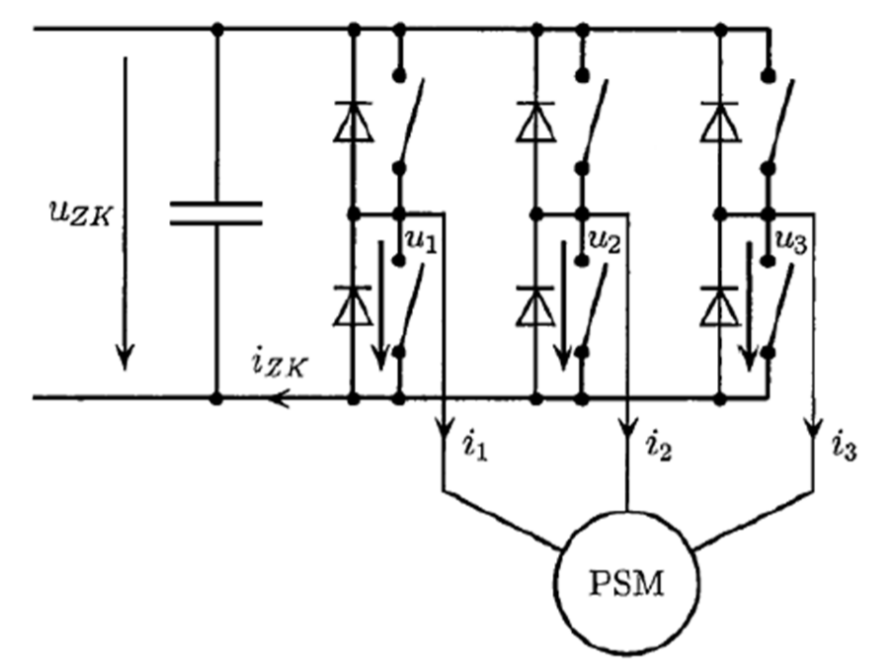
\includegraphics[scale=0.4]{1/Umrichter.png}
    \caption{Prinzipschaltbild eines Spannungszwischenkreisumrichters.}
    \label{fig:umrichter}
\end{figure}

\noindent Der Umrichter inklusive Regeleinheit ermöglicht sowohl sinusförmig wie auch blockförmig (BLDC) geführte Strangströme, Feldschwächbetrieb und eine feldorientierte Regelung. Entsprechende Sensoren zeichnen dabei die relevanten Größen auf, welche am Oszilloskop dargestellt und untersucht werden. Im Folgenden wird näher auf die einzelnen Betriebsarten und ihre Messgrößen eingegangen.

\subsection{Feldorientierte Regelung}

\begin{figure}[h!]
    \centering
    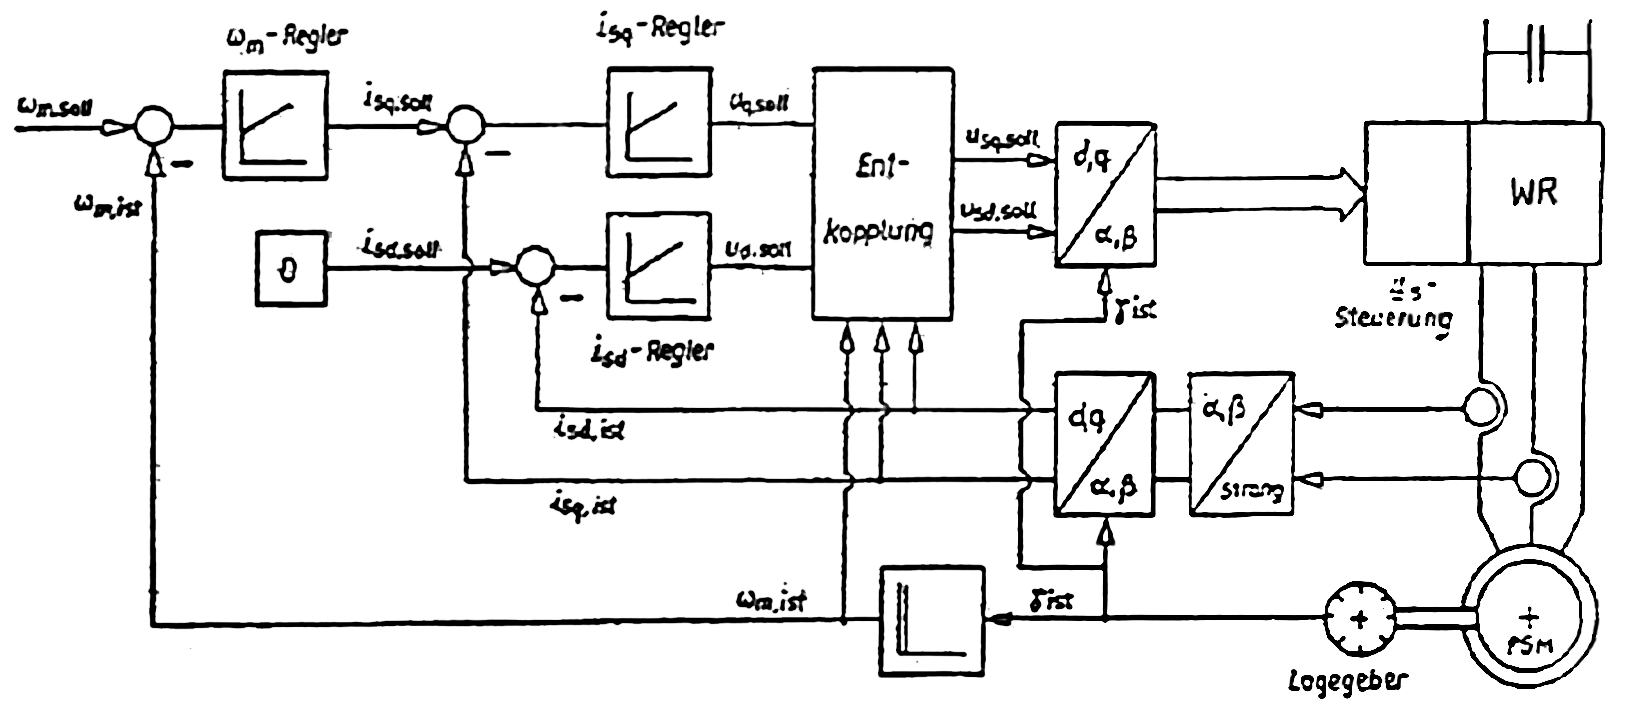
\includegraphics[scale=0.4]{1/Regelung.png}
    \caption{Blockschaltbild einer kaskadierten Regelung mit Entkopplungsnetzwerk (Entkopplung der beiden Komponenten $u_{s,q}$ und $u_{s,d}$ der Statorspannungsdifferentialgleichung).}
    \label{fig:regelkreis}
\end{figure}

\noindent Zunächst wird die hochdynamische feldorientierte Regelung betrachtet, bei der die Drehzahl der Maschine durch das Drehmoment, das entsteht, wenn eine auf den Fluss $\psi_M$ ($d$-Richtung) normal stehende $q$-Komponente des Stromes eingeprägt wird, beeinflusst werden kann:

\begin{equation}
    m_R=-\operatorname{Im}(\underline{i}_S^* \cdot \underline{\psi}_S)= i_{S,q} \cdot |\psi_M|.
\end{equation}

\noindent Der Drehzahl-Regelkreis ist dabei entsprechend Abbildung \ref{fig:regelkreis} dem Stromregler überlagert (zusätzlich kann theoretisch noch eine Lageregelung überlagert werden). Die Entkopplung sorgt dabei für eine Unabhängigkeit der Spannungen $u_d$ und $u_q$ von den jeweiligen Strömen mit gegenteiligem Index. Die $d$-Komponente des Stromes wird in dieser Betriebsart zu 0 gewählt, da sie keinen Anteil am Drehmoment hat und lediglich zu unerwünschten Kupferverlusten führen würde.\\
\noindent Der erste Versuch ist das Hochlaufen der Maschine aus dem Stillstand - zunächst mit einer Stellgrößenbeschränkung, die lediglich halbes Nennmoment zulässt (Abbildung \ref{fig:hochlauf_halb_dq}), und anschließend ohne Beschränkung (Abbildung \ref{fig:hochlauf_ganz_dq}). Deutlich erkennbar ist der lineare Anstieg der Drehzahl mit der Zeit, sobald die $q$-Stromkomponente und damit ein Drehmoment wirksam wird, was auf den Drallsatz zurückzuführen ist.
\begin{equation*}
    \tau_m\,\frac{\operatorname{d}\omega_m}{\operatorname{d}\tau}=m_R+m_L
\end{equation*}\\
Dementsprechend steigt der (Rotor-) Lagewinkel $\gamma_m$ als Integral der Drehzahl $\omega_m$ quadratisch mit Zeit $\tau$ an. Ein weiterer linearer Zusammenhang ist erkennbar, wenn man die Zeit vergleicht, die jeweils benötigt wird, um die Nenndrehzahl zu erreichen: Im ersten Fall mit Stellgrößenbeschränkung auf halben Strom dauert es auch doppelt so lange ($\approx 300 \si{\milli\second}$) als im Fall ohne Beschränkung ($\approx 150 \si{\milli\second}$).\\
Sobald die gewünschte Drehzahl erreicht ist, sinkt der Strom auf den vergleichsweise geringen Betrag, der dann nur mehr notwendig ist, um die laufenden (Reib-)\-Verluste ($m_L$) abzudecken. Die $d$-Komponente des Stromes ist dabei, wie gewünscht und erwartet, bis auf einen gewissen Wechselanteil, immer verschwindend klein.\\
Diese Schwingungen in den Strömen rühren aus dem mechanischen Aufbau der PSM her (diskrete Oberflächenmagnete, Oberwellen in der Flussverteilung). Man erkennt, dass innerhalb einer Umdrehung des Rotors sechs Perioden auftreten.\\
\noindent In Abbildung \ref{fig:hochlauf_alpha_beta} sind die um $90\degree$ phasenverschobenen Ströme während des Hochlaufs im statorfesten $\alpha,\beta$-KOS ersichtlich. Eine Umrechnung dieser gemessenen Stromkomponenten entsprechend

\begin{equation}
    \underline{i}_{S} = i_{\alpha} + \operatorname{j}i_{\beta}, \quad i_1=\operatorname{Re}(\underline{i}_{S})=i_{\alpha}, \quad i_2=\operatorname{Re}(\underline{i}_{S} \mathrm{e}^{-\operatorname{j} 120 \degree}), \quad i_3=\operatorname{Re}(\underline{i}_{S} \mathrm{e}^{-\operatorname{j} 240 \degree})
    \label{eq:umrechnung}
\end{equation}

\noindent in die jeweiligen Phasenströme liefert einen Zeitverlauf gemäß Abbildung \ref{fig:phasenstroeme_feldorientiert} (nicht direkt gemessen). Deutlich zu erkennen ist der annähernd sinusförmige Verlauf der um jeweils $120 \degree$ phasenverschobenen Ströme und die mit zunehmender Rotordrehzahl steigende Frequenz. Außerdem addieren sie sich zu jedem Zeitpunkt zu 0 (Sternschaltung ohne Mittelpunktsleiter).\\ 
\noindent Als nächster Versuch zum feldorientierten Betrieb erfolgte ein Drehzahlsprung, dessen Messgrößen in Abbildung \ref{fig:sprung_sinus} ersichtlich sind. Dabei wurde die Maschine ausgehend von $\omega_m=-1$ ohne Stellgrößenbeschränkung auf $\omega_m=1$ in die entgegengesetzte Drehrichtung beschleunigt. Man erkennt beim Start des Vorganges ein bremsendes Moment durch Einprägen einer entsprechenden $q$-Stromkomponente. Die Drehzahl sinkt, bis sie 0 erreicht, und steigt anschließend aufgrund des wirkenden Momentes zur Folge des eingeprägten Stromes wieder in die gewünschte Richtung. Die Maschine beschleunigt wieder auf die gewünschte Drehzahl und es verbleibt abermals lediglich eine geringe Stromkomponente zur Kompensation der laufenden Verluste.\\ Trägt man die Ströme jeweils auf die $x$- und $y$-Achse ($i_{\alpha}, i_{\beta}$) auf, so erhält man entsprechend Abbildung \ref{fig:stromortskurve_feldorientiert} die Stromortskurve für den feldorientierten Betrieb. Ausgehend von einem geringen Strom zur Folge der Reibung wird der Betrag des Stromes sprungartig erhöht und der Stromraumzeiger vollführt im betrachteten $\alpha,\beta$-KOS mit der Zeit eine annähernd kreisförmige Bewegung. Ist die gewünschte Drehzahl erreicht, verringert sich der Betrag (langsam) wieder auf jenen Wert, der notwendig ist, um die laufenden Verluste abzudecken.\\
Die Ortskurve entspricht dabei aufgrund der bereits erwähnten Oberwellen zu Folge des mechanischen Aufbaus nicht perfekt einem Kreis, sondern weist sechs ,,Ecken'' auf, die direkt mit den sechs zuvor beobachteten Perioden pro Rotorumdrehung in den Strömen korreliert.\\
Bei den b

 \input{\currfiledir hochlauf_halb_dq.tex}
 \input{\currfiledir hochlauf_ganz_dq.tex}
 \input{\currfiledir hochlauf_alpha_beta.tex}
 \input{\currfiledir phasenstroeme.tex}
 \input{\currfiledir drehzahlsprung.tex}
 \input{\currfiledir stromortskurve.tex}
 \input{\currfiledir brems.tex}

% \clearpage
\subsection{BLDC-Betrieb}
Der Brushless-DC Betrieb (BLDC) ist dadurch gekennzeichnet, dass zwei Stränge gegensätzlich und der dritte überhaupt nicht bestromt werden. Dadurch ergeben sich für den Stromraumzeiger nur 6 mögliche diskrete Richtungen im Abstand von jeweils \SI{60}{\degree} zueinander (vgl. links in Abbildung \ref{fig:bldc_schema}). Für die Bestimmung des Umschaltzeitpunktes ist kein teurer Lagesensor mehr nötig - es sind z.B. simple Hallelemente vollkommen ausreichend. Dieser Vorteil wird dadurch erkauft, dass aufgrund der doch recht groben Diskretisierung der möglichen Stromraumzeiger im Großteil der Rotorpositionen keine ideale Momentenausbeute möglich ist. Damit sinkt ausgehend vom maximalen Moment bei idealer Lage eines Stromraumzeigers (im rechtslauf dem Fluss $90\degree$ voreilend) mit steigendem Lagewinkel $\gamma_m$ (ist hier gleich dem Winkel zwischen Flussverkettungsraumzeiger und $\alpha$-Achse) das verfügbare Moment $m_R$ kosinusförmig, bis es beim Eintritt des Flussraumzeigers in den neuen Sektor wieder in der gleichen Form ansteigt und dann abermals das Maximum erreicht, wenn der Fluss dem nunmehr aktuellen Stromraumzeiger um genau $90\degree$ nacheilt (vgl. rechts in Abbildung \ref{fig:bldc_schema}).  

\begin{figure}[h!]
    \centering
    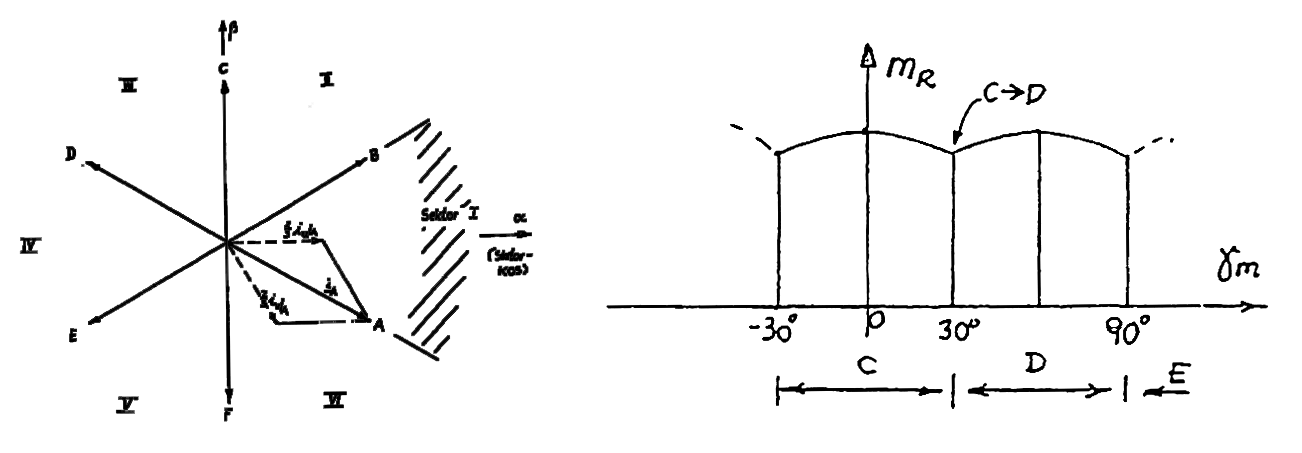
\includegraphics[scale=0.55]{2/BLDC.png}
    \caption{Diskrete Raumzeiger mit Sektoren im statorfesten KOS (links) und Momentenverlauf in Abhängigkeit der Rotorposition (rechts).}
    \label{fig:bldc_schema}
\end{figure}

\noindent Im Zuge eines erneuten Drehzahlsprunges wurden die Ströme in dieser Betriebsart gemessen. Diese sind als Stromortskurve in Abbildung \ref{fig:stromortskurve_bldc} dargestellt und zeigen die erwarteten diskreten Stromraumzeiger. Die abweichenden Stromraumzeiger, die mitten in den Sektoren zu liegen kommen, sind auf die nicht ideale Umschaltung der Stromblöcke zurückzuführen, auf die später genauer eingegangen wird (vgl. dazu Abbildung \ref{fig:phasen_genauer}).
\noindent Weiters ist der entsprechende Zeitverlauf der Messgrößen dieses Versuches in Abbildung \ref{fig:sprung_bldc} dargestellt. Eine Umrechnung der $\alpha, \beta$-Komponenten des Statorstromes in die entsprechenden Strangströme gemäß Gl. \ref{eq:umrechnung} liefert wiederum deren zeitlichen Verlauf in Abbildung \ref{fig:phasenstroeme_bldc} (wieder berechnet, nicht direkt gemessen).\\
In beiden Diagrammen sind deutlich die diskreten Werte der Ströme und auch die für den BLDC-Betrieb charakteristische Schaltfolge zu erkennen, sowie die Tatsache, dass sich auch hier die Summe der Strangströme stets zu 0 addiert.\\
Beim Drehzahlsprung ist im Umkehrpunkt der Drehrichtung auch der Lagewinkel $\gamma_m$ zufällig gleich 0, und man erkennt deswegen sehr gut, dass in diesem Fall (Fluss $\psi_M$ zeigt in die $\alpha$-Achse bzw. in Richtung des ersten Stranges) der Stromraumzeiger $F$ ideal ist, da dieser dem Fluss zu diesem Zeitpunkt genau $90\degree$ nacheilt (Linkslauf). Dieser Zeiger korrespondiert mit der negativen $\beta$-Achse, demzufolge ist auch der negative $i_{\beta}$ maximal und $i_{\alpha}$ gleich 0. Dies spiegelt sich ebenso in den Strangströmen wider, wo entsprechend $i_1$ gleich 0, $i_2$ negativ und $i_3$ positiv ist.\\
Weiters ist anzumerken, dass es in den Strangströmen bei höheren Drehzahlen zu Stromeinbrüchen aufgrund der Schaltvorgänge kommt. In Abbildung \ref{fig:phasen_genauer} ist der Verlauf der Strangströme genauer dargestellt und dieser Umstand neben jenem, dass die Stromschaltung nicht ideal mit unendlich steiler Flanke, sondern physikalisch mit exponentiellem Verlauf erfolgt ($R-L$-Glied bzw. $PT_1$), sehr gut erkennbar.\\
\noindent Abschließend wird ein weiterer Drehzahlsprung betrachtet, diesmal jedoch im $d,q$-KOS (vgl. Abbildung \ref{fig:umkehr_bldc_dq}). Zu sehen ist der qualitativ erwartete Verlauf des $q$-Stromes entsprechend des rechten Teils der Abb. \ref{fig:bldc_schema}, da der Fluss konstant und das wellige Moment damit proportional zur $q$-Stromkomponente ist. Dementsprechend ist im BLDC-Betrieb auch der $d$-Strom nur mehr dort 0, wo die Momentenausbeute ideal ist und zeigt andernfalls ein Sägezahn-Verhalten: Bei jedem Umschaltvorgang wechselt die Projektion des diskreten Stromraumzeigers auf die $d$-Achse ihr Vorzeichen und nimmt betraglich ab, bis sie verschwindet, um dann mit dem Lagewinkel wieder bis zur nächsten Umschaltung betraglich zu steigen. Betrachtet man den maximalen Einbruch des Momentes und folglich der $q$-Stromkomponente im idealen Fall, so beträgt dieser $1-\cos(30\degree) \approx 0.13$. In der Messung tritt ein Einbruch von $\approx 0.25$ auf, also fast ein doppelt so großer Wert. Dies ist wieder auf die endliche Schaltzeit zurückzuführen.

\input{\currfiledir stromortskurve.tex}
\input{\currfiledir sprung_bldc.tex}
\input{\currfiledir phasenstroeme.tex}
\input{\currfiledir phasen_genauer.tex}
\input{\currfiledir umkehr_bldc_dq.tex}


\clearpage 

\subsection{Feldschwächbetrieb} 
%Die PSM ist schlecht feldschwächbar! 
%:D
Ziel des Feldschächbetriebs ist es, die Maschine über die Nenndrehzahl $n_N$ hinaus zu betreiben, ohne dabei die Statornennspannung $U_{S,N}$ zu überschreiten. Wird eine negative $d$-Komponente des Statorstromes $\underline{i}_S$ eingeprägt, bewirkt das einen Fluss $\Phi_d$ der dem Fluss $\Phi_M$ des Permanentmagneten entgegengesetzt ist (Feldschwächung); siehe Statorflussverkettungsgleichung:\\
\begin{equation*}
     \underline{\psi}_S= \underline{\psi}_M+l_S\,\underline{i}_S
\end{equation*}
Durch den geringeren Flussbetrag sinkt gemäß der Statorspannungsgleichung (stationäre Verhältnisse)
\begin{equation*}
     \underline{u}_S=r_S\,\underline{i}_S+\frac{\mathrm{d}\underline{\psi}_S}{\mathrm{d}\tau}+\mathrm{j}\,\omega_K\,\underline{\psi}_S
\end{equation*}
die induzierte Spannung, und damit die Außenleiterspannung.\\
Allerdings leistet die $d$-Komponente des Stromes keinen Beitrag zum Drehmoment, muss jedoch vom Umrichter zur Verfügung gestellt werden. Für einen Maximalbetrag (begrenzt durch Umrichter) des Stromraumzeigers, bedeutet dies jedoch eine Verringerung des Drehmomentes der Maschine und damit ihrer abgegebenen mechanischen Leistung.\\
Für den Versuch wurde bei Nenndrehzahl ein bezogener Strom $i_d$ in negative Richtung eingeprägt. Dabei wurde die Außenleiterspannung $U_{AL}$ gemessen. Die Messwerte sind in Tabelle \ref{tab:PSM_feldschwaech} dargestellt.

\begin{table}[!ht]
\centering% Tabelle zu Kurzschluss
    \begin{tabular}{|l|c|}
    \hline
    $i_d [1]$ & $U_{AL} [V]$ \\ \hline
    0         & 107          \\ \hline
    -0.1      & 103          \\ \hline
    -0.2      & 99           \\ \hline
    -0.3      & 96           \\ \hline
    -0.4      & 92           \\ \hline
    -0.5      & 88           \\ \hline
    \end{tabular}
    \caption{Messwerte zum Feldschwächbetrieb}
    \label{tab:PSM_feldschwaech}
\end{table}
\noindent In Abbildung \ref{fig:feldschwaech} sind links die gemessenen Punkte dargestellt. Rechts ist die aus den Messdaten extrapolierte Gerade eingezeichnet, zusammen mit dem Wert
\begin{equation*}
    i_{d,0} = -2.855,
\end{equation*}
bei der die extrapolierte Außenleiterspannung Null wird. Man kann daraus auf die bezogene Induktivität der Maschine in $d$-Richtung $l_d=x_d$ schließen:
\begin{equation*}
    x_d = \frac{1}{|i_{d,0}|} \approx 0.35,
\end{equation*}
was dem typischen Wert einer PSM von $x_d \approx \frac{1}{3}$ entspricht.
\input{\currfiledir aussenleiterspannung.tex}
\section{Anhang}
Lorem ipsum dolor sit amet, consectetur adipiscing elit. Mauris fringilla suscipit faucibus. Duis tincidunt, augue et dapibus lacinia, tortor mi viverra sapien, non ullamcorper odio risus a mauris. Maecenas at libero et mauris scelerisque sollicitudin quis sed orci. Donec congue ante felis, rutrum commodo lorem auctor quis. In consequat luctus turpis et vulputate. In sit amet rhoncus risus, porta imperdiet ex. Morbi neque lacus, consectetur quis dictum quis, pulvinar ac urna. Aliquam in dolor ut erat facilisis fringilla. Sed molestie commodo est.

Mauris sit amet eros sem. Donec quam massa, luctus ut nunc at, dignissim ornare augue. Aenean sagittis consequat nulla quis facilisis. Duis ultricies laoreet dui, ut condimentum arcu sodales sit amet. Nullam efficitur tellus vel faucibus scelerisque. Duis varius felis vitae eros maximus vestibulum. In porttitor pellentesque tellus, vel placerat orci. Phasellus consequat libero purus, sit amet semper ipsum fermentum non. Quisque rutrum sapien lectus, at faucibus eros egestas eget. Nulla id nisi tortor. Morbi porttitor interdum porta.

Morbi porta dolor metus, eget hendrerit justo ullamcorper ut. Vivamus commodo, arcu quis finibus eleifend, odio sem dignissim orci, nec pellentesque sapien metus at tortor. Sed dictum lectus suscipit imperdiet ultrices. Proin tellus neque, ornare sed mattis vel, faucibus at turpis. Lorem ipsum dolor sit amet, consectetur adipiscing elit. Morbi sit amet condimentum risus, nec lobortis sem. Donec molestie vel dui in egestas. Quisque tellus nisl, suscipit at viverra eget, aliquam eu est. Nam cursus nunc ultrices, pulvinar lorem vel, ullamcorper ante. Nunc sed dolor nec tellus commodo vehicula.

Phasellus id arcu sed enim sodales fringilla at nec metus. Mauris vel nibh et nibh bibendum gravida ut at metus. Sed bibendum, dui nec congue sodales, quam urna gravida lorem, sed vestibulum velit mi nec lorem. Quisque placerat congue ullamcorper. Vestibulum sollicitudin enim at risus gravida suscipit. Maecenas blandit consectetur enim, sed maximus diam dignissim at. Nam venenatis erat eleifend velit posuere accumsan. Nunc bibendum felis ac elit posuere venenatis. Suspendisse aliquet quam magna. Aenean quis ante posuere, interdum quam ut, accumsan ex.

Fusce molestie lacinia maximus. Suspendisse eget ex nec orci ullamcorper euismod auctor sed dui. Vivamus iaculis egestas tellus non consectetur. Sed dapibus vitae felis in gravida. Donec sapien sem, euismod et tincidunt egestas, bibendum eget odio. Nulla sed sapien efficitur, mattis metus ac, aliquam leo. Integer consequat bibendum turpis, at rhoncus purus sodales eget. Aenean quis accumsan velit.
\end{document}

